\ylDisplay{Elektriskeem} % Ülesande nimi
{EFO žürii} % Autor
{piirkonnavoor} % Voor
{2019} % Aasta
{P 7} % Ülesande nr.
{3} % Raskustase
{
% Teema: Elektriõpetus

\ifStatement
Kõigi vooluringis olevate takistite takistus on sama suur. Kui suur on takisti takistus, kui vooluallika pinge $U = 3$ $V$ korral näitab ampermeeter voolutugevuseks $I = 1$ $A$.
\begin{center}
	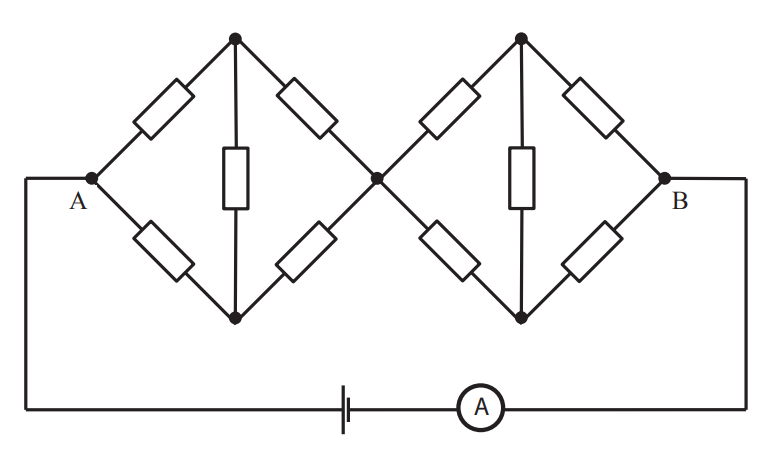
\includegraphics[width=0.5\linewidth]{2019-v2p-07-yl.png}
\end{center}
\fi

\ifHint
Ruudu kaks vastastippu (ülemine ja alumine) on ka takistiga ühendatud, kuid selles takistis voolu ei ole. Skeemi ülemine ja alumine haru on sümmeetrilised, seega on pinge nii ülemise kui ka alumise haru esimese takisti otstel sama suur ning vertikaalselt paikneva takisti otstel pinge puudub. Seetõttu ei teki vertikaalselt paiknevas takistis elektrivoolu ning selle takisti takistust ei ole tarvis arvestada. Ruudu ülemiste takistite jada ja alumiste takistite jada on ühendatud rööbiti.
\fi


\ifSolution
Vooluringis on neli takistit ühendatud ruudukujuliselt ruudu erinevatesse külgedesse ning üks takisti paikneb ruudu diagonaalil. Selliseid ruute on jadamisi ühendatud kaks. Nii ruudu ülemises kui ka ruudu alumises kahes küljes on kaks takistit ühendatud jadamisi ning kummagi jada takistus on $R_j = R + R = 2R$. Ruudu kaks vastastippu (ülemine ja alumine) on ka takistiga ühendatud, kuid selles takistis voolu ei ole. Skeemi ülemine ja alumine haru on sümmeetrilised, seega on pinge nii ülemise kui ka alumise haru esimese takisti otstel sama suur ning vertikaalselt paikneva takisti otstel pinge puudub. Seetõttu ei teki vertikaalselt paiknevas takistis elektrivoolu ning selle takisti takistust ei ole tarvis arvestada. Ruudu ülemiste takistite jada ja alumiste takistite jada on ühendatud rööbiti. Seega on ruudu kogutakistus $R_r =\frac{2R}{2}= R$. Kaks samasugust ruutu on ühendatud jadamisi. Vooluringi kogutakistus on seega
\begin{center}
$R_k = R + R = 2R$.
\end{center}
Ohmi seadusest
\begin{center}
$I = \frac{U}{R_k}$ 
\end{center}
saame, et
\begin{center}
$R_k = \frac{U}{I} = 3$ $\Omega$ 
\end{center}
ning
\begin{center}
$R = \frac{R_k}{2} = 1,5$ $\Omega$.
\end{center}
\fi
}